\documentclass[11pt]{article}

\newcommand{\yournames}{Apoorva Jarmale, Kaavya Gowthaman, Oj Sindher, Sarang Pande, Vartika Tewari}

\def\comments{0}

%format and packages
\usepackage{hyperref}
\usepackage{biblatex}

\addbibresource{references.bib}

\usepackage{url}
%\usepackage{algorithm, algorithmic}
\usepackage{algpseudocode}
\usepackage{amsmath, amssymb, amsthm}
\usepackage{enumerate}
\usepackage{enumitem}
\usepackage{framed}
\usepackage{verbatim}
\usepackage[margin=1.1in]{geometry}
\usepackage{microtype}
\usepackage{kpfonts}
\usepackage{palatino}
\usepackage{graphicx}
	\DeclareMathAlphabet{\mathtt}{OT1}{cmtt}{m}{n}
	\SetMathAlphabet{\mathtt}{bold}{OT1}{cmtt}{bx}{n}
	\DeclareMathAlphabet{\mathsf}{OT1}{cmss}{m}{n}
	\SetMathAlphabet{\mathsf}{bold}{OT1}{cmss}{bx}{n}
	\renewcommand*\ttdefault{cmtt}
	\renewcommand*\sfdefault{cmss}
	\renewcommand{\baselinestretch}{1.05}
\usepackage[usenames,dvipsnames]{xcolor}
\definecolor{DarkGreen}{rgb}{0.15,0.5,0.15}
\definecolor{DarkRed}{rgb}{0.6,0.2,0.2}
\definecolor{DarkBlue}{rgb}{0.2,0.2,0.6}
\definecolor{DarkPurple}{rgb}{0.4,0.2,0.4}
\hypersetup{
	linktocpage=true,
	colorlinks=true,				% false: boxed links; true: colored links
	linkcolor=DarkBlue,		% color of internal links
	citecolor=DarkBlue,	% color of links to bibliography
	urlcolor=DarkBlue,		% color of external links
}

\usepackage[boxruled,vlined,nofillcomment]{algorithm2e}
	\SetKwProg{Fn}{Function}{\string:}{}
	\SetKwFor{While}{While}{}{}
	\SetKwFor{For}{For}{}{}
	\SetKwIF{If}{ElseIf}{Else}{If}{:}{ElseIf}{Else}{:}
	\SetKw{Return}{Return}

\newcommand{\red}[1]{ {\color{red} #1} }


%enclosure macros
\newcommand{\paren}[1]{\ensuremath{\left( {#1} \right)}}
\newcommand{\bracket}[1]{\ensuremath{\left\{ {#1} \right\}}}
\renewcommand{\sb}[1]{\ensuremath{\left[ {#1} \right\]}}
\newcommand{\ab}[1]{\ensuremath{\left\langle {#1} \right\rangle}}

%probability macros
\newcommand{\ex}[2]{{\ifx&#1& \mathbb{E} \else \underset{#1}{\mathbb{E}} \fi \left[#2\right]}}
\newcommand{\pr}[2]{{\ifx&#1& \mathbb{P} \else \underset{#1}{\mathbb{P}} \fi \left[#2\right]}}
\newcommand{\var}[2]{{\ifx&#1& \mathrm{Var} \else \underset{#1}{\mathrm{Var}} \fi \left[#2\right]}}

%useful CS macros
\newcommand{\poly}{\mathrm{poly}}
\newcommand{\polylog}{\mathrm{polylog}}
\newcommand{\zo}{\{0,1\}}
\newcommand{\pmo}{\{\pm1\}}
\newcommand{\getsr}{\gets_{\mbox{\tiny R}}}
\newcommand{\card}[1]{\left| #1 \right|}
\newcommand{\set}[1]{\left\{#1\right\}}
\newcommand{\negl}{\mathrm{negl}}
\newcommand{\eps}{\varepsilon}
\DeclareMathOperator*{\argmin}{arg\,min}
\DeclareMathOperator*{\argmax}{arg\,max}
\newcommand{\eqand}{\qquad \textrm{and} \qquad}
\newcommand{\ind}[1]{\mathbb{I}\{#1\}}
\newcommand{\sslash}{\ensuremath{\mathbin{/\mkern-3mu/}}}

%info theory macros
\newcommand{\SD}{\mathit{SD}}
\newcommand{\sd}[2]{\SD\left( #1 , #2 \right)}
\newcommand{\KL}{\mathit{KL}}
\newcommand{\kl}[2]{\KL\left(#1 \| #2 \right)}
\newcommand{\CS}{\ensuremath{\chi^2}}
\newcommand{\cs}[2]{\CS\left(#1 \| #2 \right)}
\newcommand{\MI}{\mathit{I}}
\newcommand{\mi}[2]{\MI\left(~#1~;~#2~\right)}

%mathbb
\newcommand{\N}{\mathbb{N}}
\newcommand{\R}{\mathbb{R}}
\newcommand{\Z}{\mathbb{Z}}
%mathcal
\newcommand{\cA}{\mathcal{A}}
\newcommand{\cB}{\mathcal{B}}
\newcommand{\cC}{\mathcal{C}}
\newcommand{\cD}{\mathcal{D}}
\newcommand{\cE}{\mathcal{E}}
\newcommand{\cF}{\mathcal{F}}
\newcommand{\cL}{\mathcal{L}}
\newcommand{\cM}{\mathcal{M}}
\newcommand{\cO}{\mathcal{O}}
\newcommand{\cP}{\mathcal{P}}
\newcommand{\cQ}{\mathcal{Q}}
\newcommand{\cR}{\mathcal{R}}
\newcommand{\cS}{\mathcal{S}}
\newcommand{\cU}{\mathcal{U}}
\newcommand{\cV}{\mathcal{V}}
\newcommand{\cW}{\mathcal{W}}
\newcommand{\cX}{\mathcal{X}}
\newcommand{\cY}{\mathcal{Y}}
\newcommand{\cZ}{\mathcal{Z}}


%theorem macros
\newtheorem{thm}{Theorem}
\newtheorem{lem}[thm]{Lemma}
\newtheorem{fact}[thm]{Fact}
\newtheorem{clm}[thm]{Claim}
\newtheorem{rem}[thm]{Remark}
\newtheorem{coro}[thm]{Corollary}
\newtheorem{prop}[thm]{Proposition}
\newtheorem{conj}[thm]{Conjecture}
	\theoremstyle{definition}
\newtheorem{defn}[thm]{Definition}

\theoremstyle{theorem}
\newtheorem{prob}{Problem}
\newtheorem{sol}{Solution}
\newtheorem{ques}{Question}
\newtheorem{ans}{Answer}


\definecolor{cit}{rgb}{0.05,0.2,0.45} 
\newcommand{\solution}{\medskip\noindent{\color{DarkBlue}\textbf{Solution:}}}
\newcommand{\response}{\medskip\noindent{\color{DarkBlue}\textbf{Response:}}}
\title{Exploring Variational Auto-Encoders for Topic Modelling}
\author{Apoorva Jarmale,Kaavya Gowthaman,Oj Sindher,Sarang Pande,Vartika Tewari}
\begin{document}
\maketitle
\begin{center}
    \subsection*{Project Milestone Report (DS 5230: USML | Spring 2021)}
\end{center}
%{\Large 
%\begin{center}{CS 5230: Unsupervised Machine Learning} --- Spring 2021 \end{center}}

%{\large
%\vspace{10pt}
%\noindent Project Milestone Report\  \vspace{2pt}}

%\bigskip
%{\large
%\noindent Names: \yournames \vspace{2pt}}

%\vspace{15pt}

%\begin{ques} Project Milestone Report
%\end{ques}

\abstract
Topic models are one of the most popular methods for learning representations of
text, but a major challenge is that any change to the topic model requires mathematically deriving a new inference algorithm. In this project, we implement a model called ProdLDA, that replaces the mixture model in LDA with a product
of experts. This model tackles the problems caused for autoencoding variational Bayes by the Dirichlet prior and by component collapsing. We find that Autoencoded Variational Inference For Topic Model matches traditional methods in accuracy with much better inference time. The data used for the analysis is 20 Newsgroup data set. The 20 Newsgroups data set is a collection of approximately 20,000 newsgroup documents, partitioned (nearly) evenly across 20 different newsgroups. Each sub directory in the bundle represents a newsgroup; each file in a sub directory is the text of some newsgroup document that was posted to that newsgroup. In project milestone report, we are implementing variational autoencoder(standard LDA) on MNIST data set.\\
 

\section{Introduction}

\response

The variational inference methods tries to solve the major challenge of applying topic models to the text data, which is the computational cost of computing the posterior distribution, as posterior inference over the hidden variables $\theta$ and z is intractable due to the coupling between the $\theta$ and $\beta$ under the multinomial assumption (Dickey, 1983). Though these inference methods have been used and developed by a large body of work, they posses a common issue when applying them to new models, that is, it relies on the practitioner’s ability to derive the closed form updates, which can be impractical and sometimes impossible. This has motivated the development of black-box inference methods (Ranganath et al., 2014; Mnih & Gregor, 2014; Kucukelbir et al., 2016; Kingma & Welling, 2014; Srivastava et al., 2017). 

Autoencoding variational Bayes (AEVB) is a black-box inferencing method which trains an inference network (Dayan et al., 1995) to map a document to an approximate posterior distribution, though practically AEVB faces several challenges, such as, we need to determine the reparameterization function for q($\theta$) in order to use the “reparameterization trick” Rezende et al. (2014), which is essential because it allows the backpropagation of gradient to flow from deterministic nodes instead of the random nodes. The ProdLDA model, which is advancement of AEVB makes them stable, and it also has been able to address the drawbacks of implementing topic models by either using variational inference methods such as mean field or Gibbs sampling methods, as shown by Srivastava et al. (2017) in their research paper where they presented ProdLDA model for the first time. It is very interesting that how changing one assumption in LDA model results in drastic improvement in topic coherence. Basically, ProdLDA model just replaces the mixture assumption at the word-level in LDA with a weighted product of experts. In other words, ProdLDA is an instance of the exponential-family PCA (Collins et al., 2001) class, and relates to the exponential-family harmoniums (Welling et al., 2004) but with non-Gaussian priors. \\

We would be implementing the ProdLDA model which is a very effective AEVB inference method for text data. The model described promises advantages like topic coherence, computational efficiency, and a Black-box methodology i.e. it does not require rigorous mathematical derivations to handle changes in the model, and can be easily applied to a wide-range of topic models.

\section{Background}

Topic Models are used to assign topics to documents. There are various techniques for topic modelling , some of the earliest techniques include  probabilistic latent semantic analysis (PLSA)\cite{plsa}, Latent Dirichlet allocation (LDA)\cite{blei2003latent}. Latent Drichlet Allocation assumes the generative process of the data. Each document contains some topics and each word can be mapped to one of the document's topics. Other topic models are generally extensions of LDA. 
\begin{figure}
  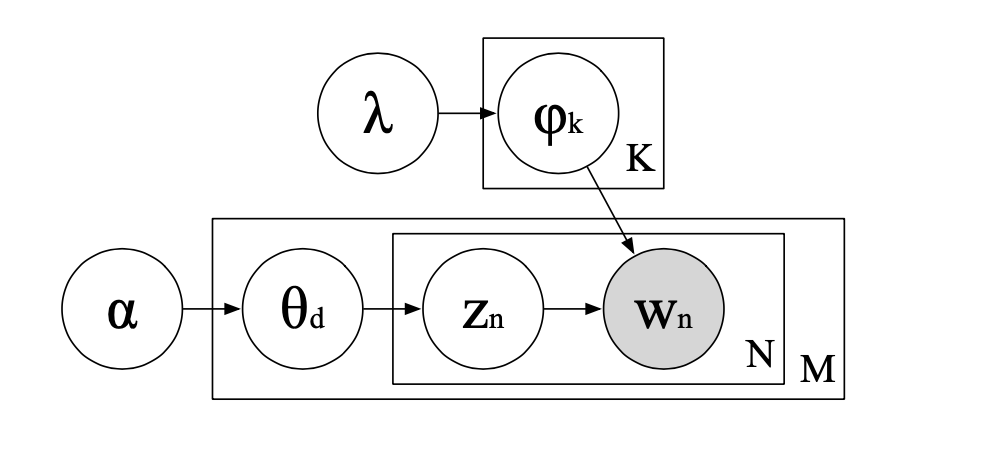
\includegraphics[width=\linewidth]{lda}
  \caption{Plate diagram for LDA. Nodes show random variables, lines show
(possible) probabilistic dependence, rectangles show repetition, and shading shows
observation}
  \label{fig:ldaplate}
\end{figure}

In this project we will focus on ProdLDA\cite{prodlda} which uses Variational Autoencoders to do topic modeling. \subsection{Variational Inference using Autoencoders}
\subsubsection{Autoencoders}
Autoencoders are neural networks which tries to recreate the input as its output. It consists of two parts encoder and decoder. The encoder maps the input to an embedding and the decoder maps the embedding to the reconstructed input. They are mostly used for dimentionality reduction or feauture learning. 
\subsubsection{Variational Autoencoders\cite{vae}}
To make a generative model we add regularisation in the training process of the autoencoder. So instead of encoding an input as a single point, we encode it as a distribution over the latent space. This variation now uses the point sampled from a distribution for the decoding process. 

\begin{figure}
  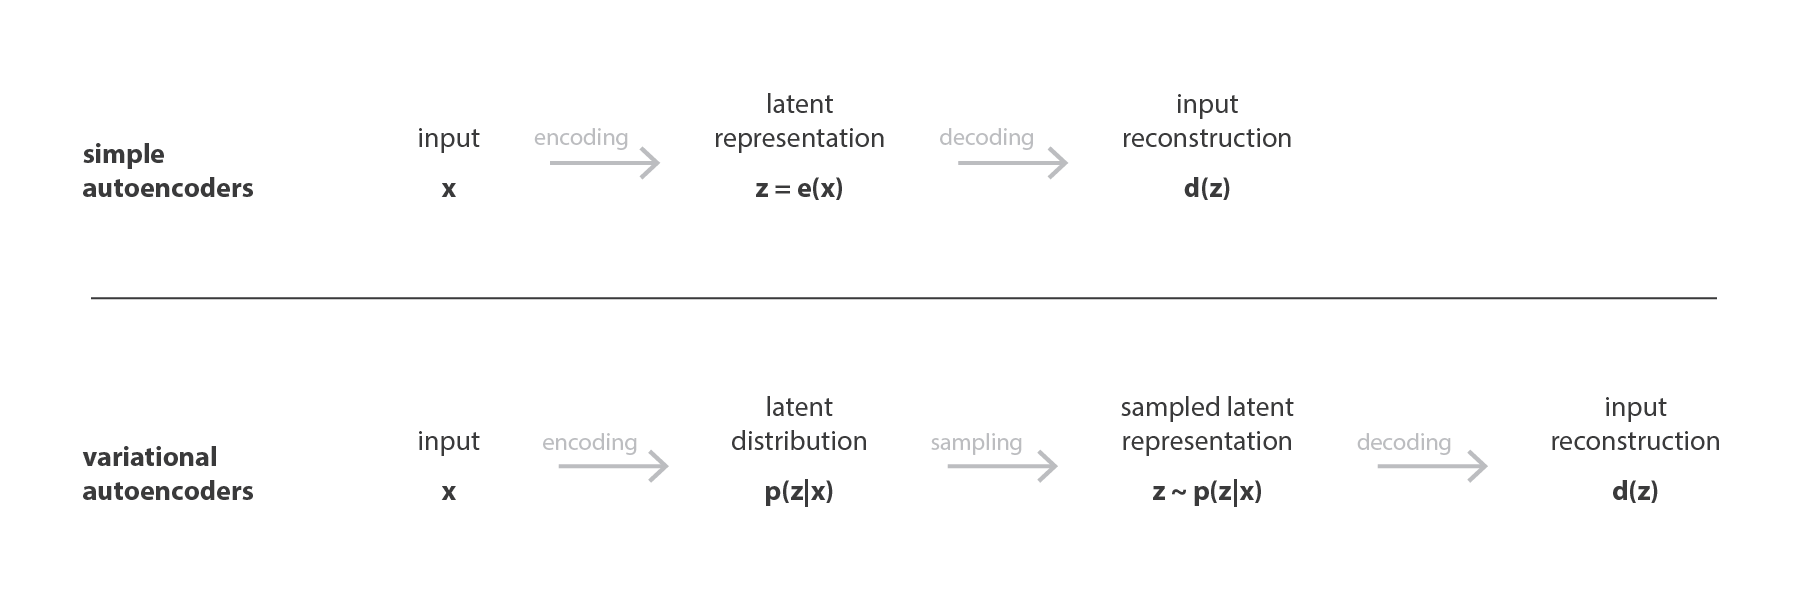
\includegraphics[width=\linewidth]{vaes.png}
  \caption{Difference between autoencoder and variational autoencoder}
  \label{fig:aevsvae}
\end{figure}

\textbf{ELBO Loss}: 
The loss function for the VAE is called the ELBO.
\begin{align*} min \mathbb{E}_{q}\log p(z)- \mathbb{E}_{q}\log p(x|z)\end{align*} The first term is the KL divergence. The second term is the reconstruction term.

%Give more detailed background information. Describe any analysis methods that you are going to use (with equations), and how they apply to your problem.

\section{Preliminary Results} 
For the preliminary results, we worked on understanding and running a simple variational autoencoder. VAE implemented here uses the setup found in most VAE papers:a multivariate Normal distribution for the conditional distribution of the latent vectors given and input image and a multivariate Bernoulli distribution for the conditional distribution of images given the latent vector. Using a Bernoulli distribution, the reconstruction loss (negative log likelihood of a data point in the output distribution) reduces to the pixel-wise binary cross-entropy. This VAE has been used with the MNIST dataset. We learnt that in this case, a convolutional encoder and decoder,  gives better performance than fully connected versions that have the same number of parameters.
\\ Following is the parameter setting :\\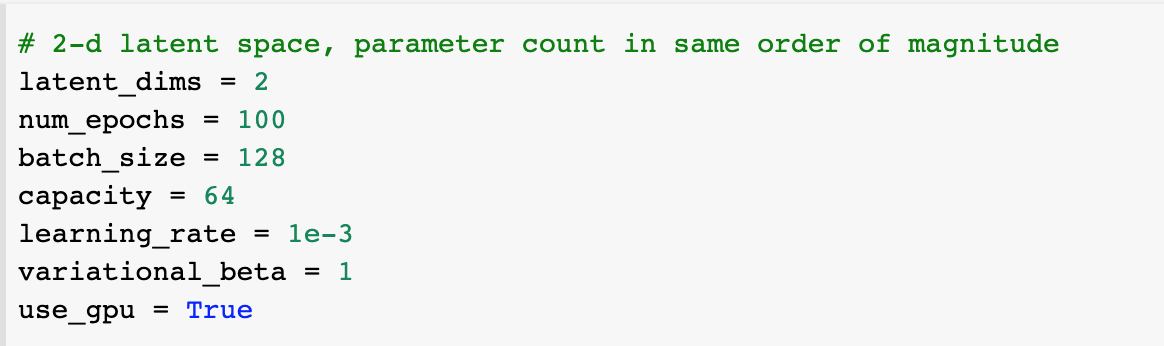
\includegraphics[width=15cm, height=4cm]{Param.png}\\\\As a preliminary dataset, we have considered MNIST. MNIST images show digits from 0-9 in 28x28 grayscale images. We do not center them at 0, because we will be using a binary cross-entropy loss that treats pixel values as probabilities in [0,1]. We create both a training set and a test set as follows :\\\\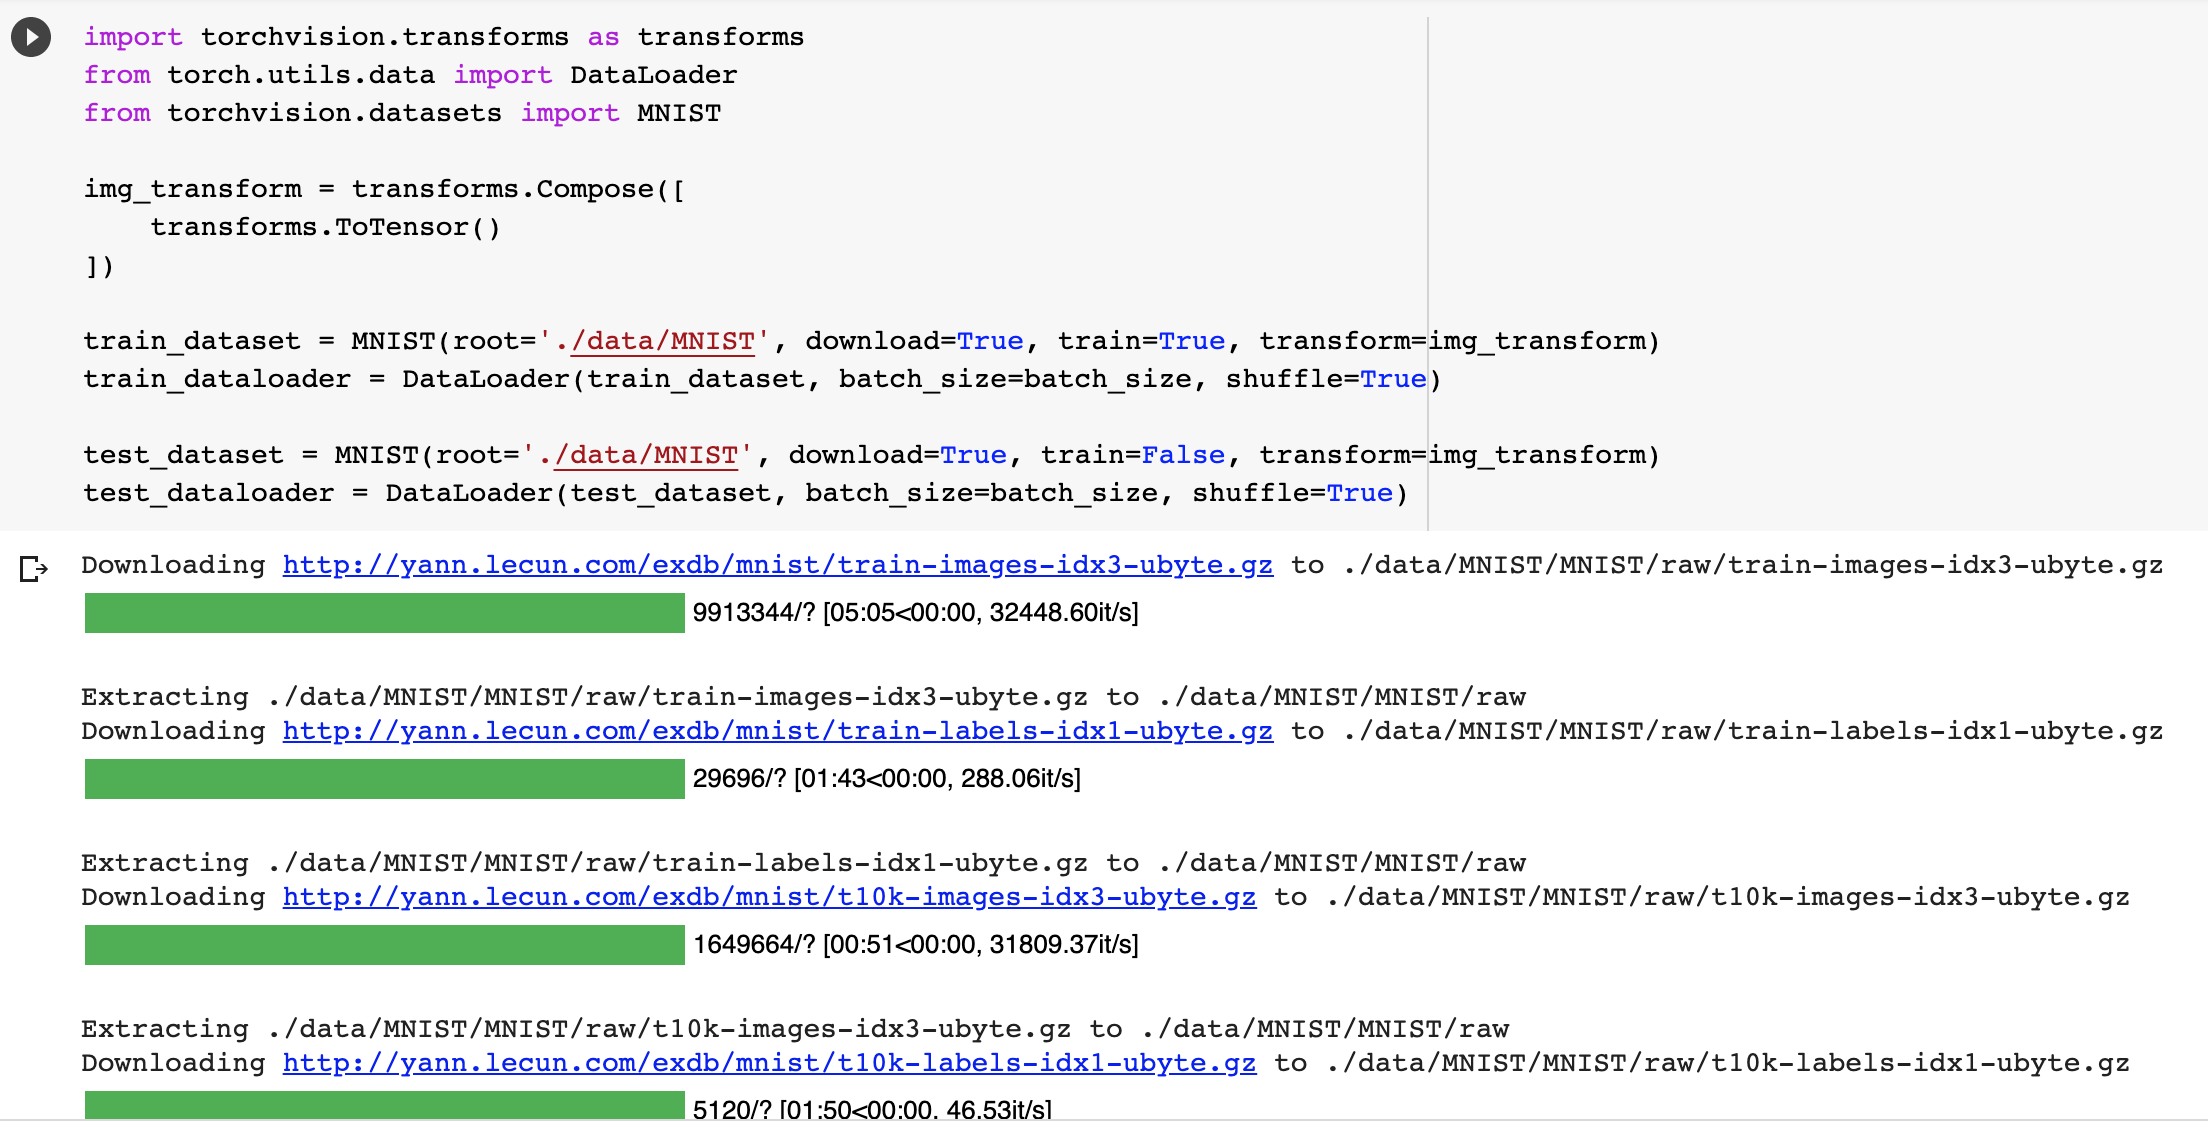
\includegraphics[width=15cm, height=8cm]{data-load.png}\\\\\The encoder is a neural network. Its input is a datapoint x, its output is a hidden representation z, and it has weights and biases $\theta$. \\The encoder learns an efficient compression of the data into this lower-dimensional space.Suppose we denote the encoder  q$_\theta$(z$\mid$ x). We note that the lower-dimensional space is stochastic: the encoder outputs parameters to  q$_\theta$(z$\mid$ x), which is a Gaussian probability density. We can sample from this distribution to get noisy values of the representations z.\\The decoder is another neural net. Its input is the representation z, it outputs the parameters to the probability distribution of the data, and has weights and biases $\theta$. The decoder is denoted by p$_\theta$(x$\mid$ z).\\\\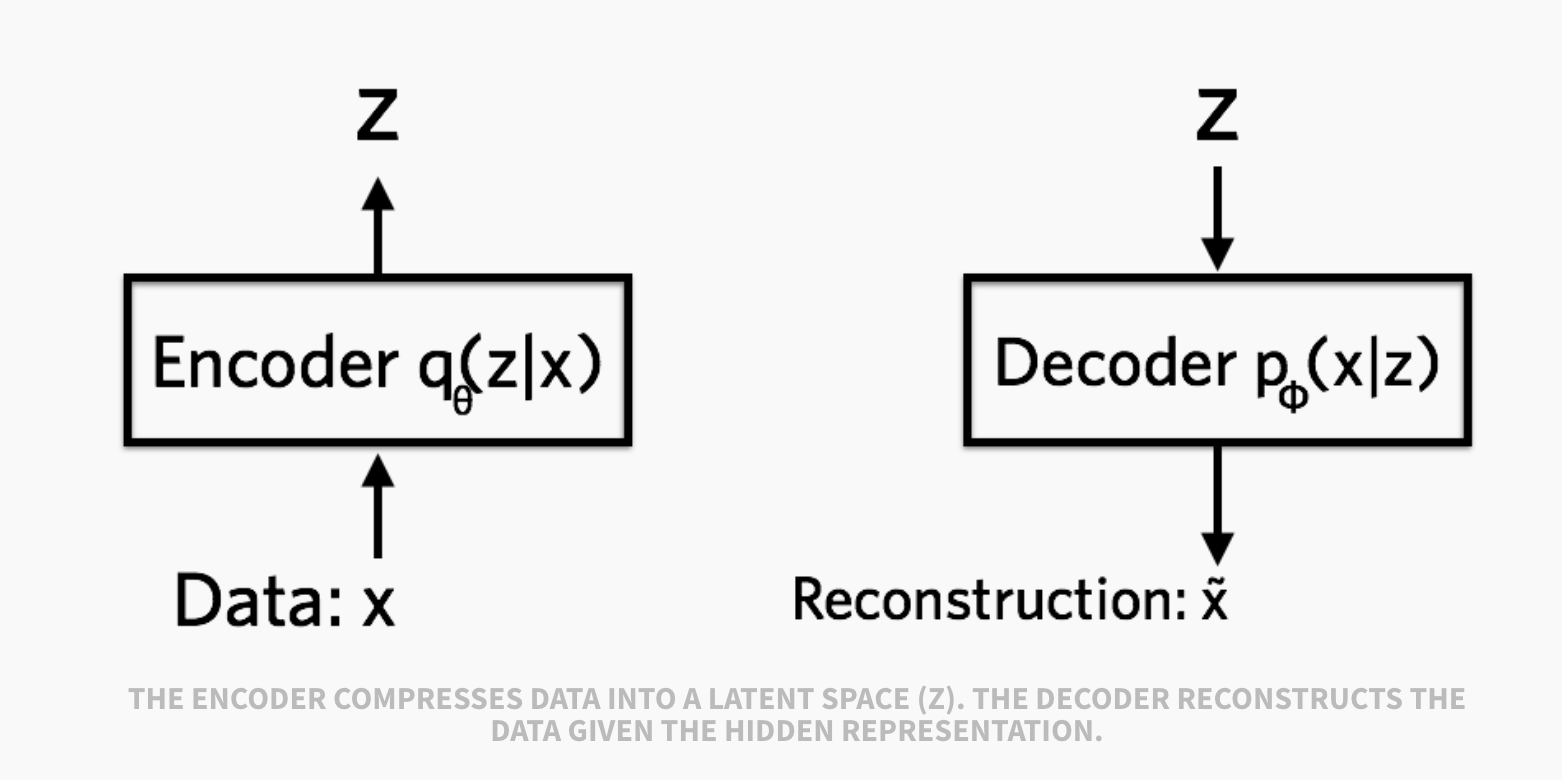
\includegraphics[width=15cm, height=8cm]{encoder-decoder-dia.png}\\\\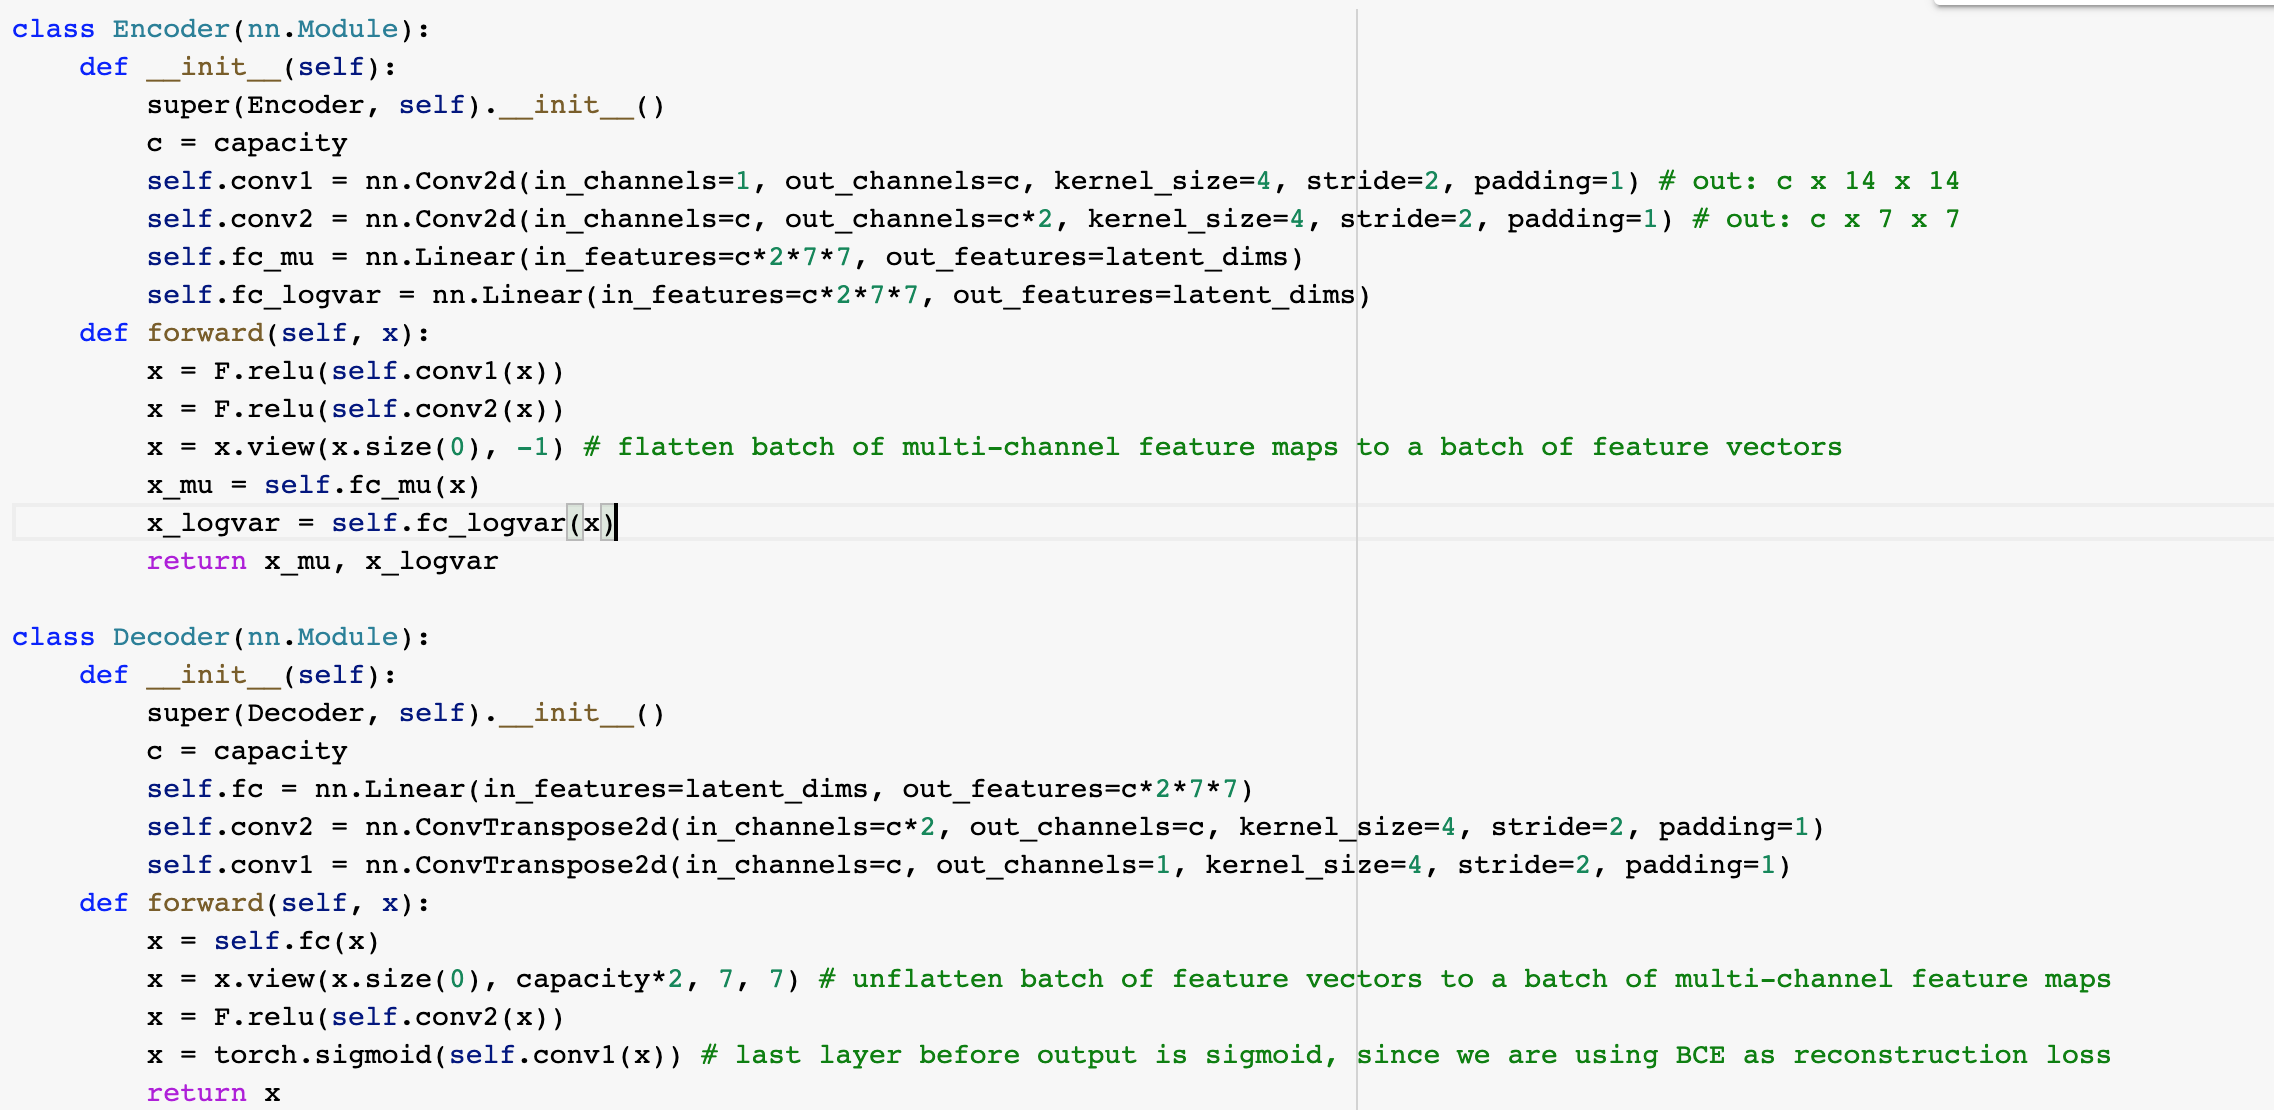
\includegraphics[width=15cm, height=8cm]{encoder-decoder.png}\\The VAE is implemented with the reparametrization trick shown as follows :\\\\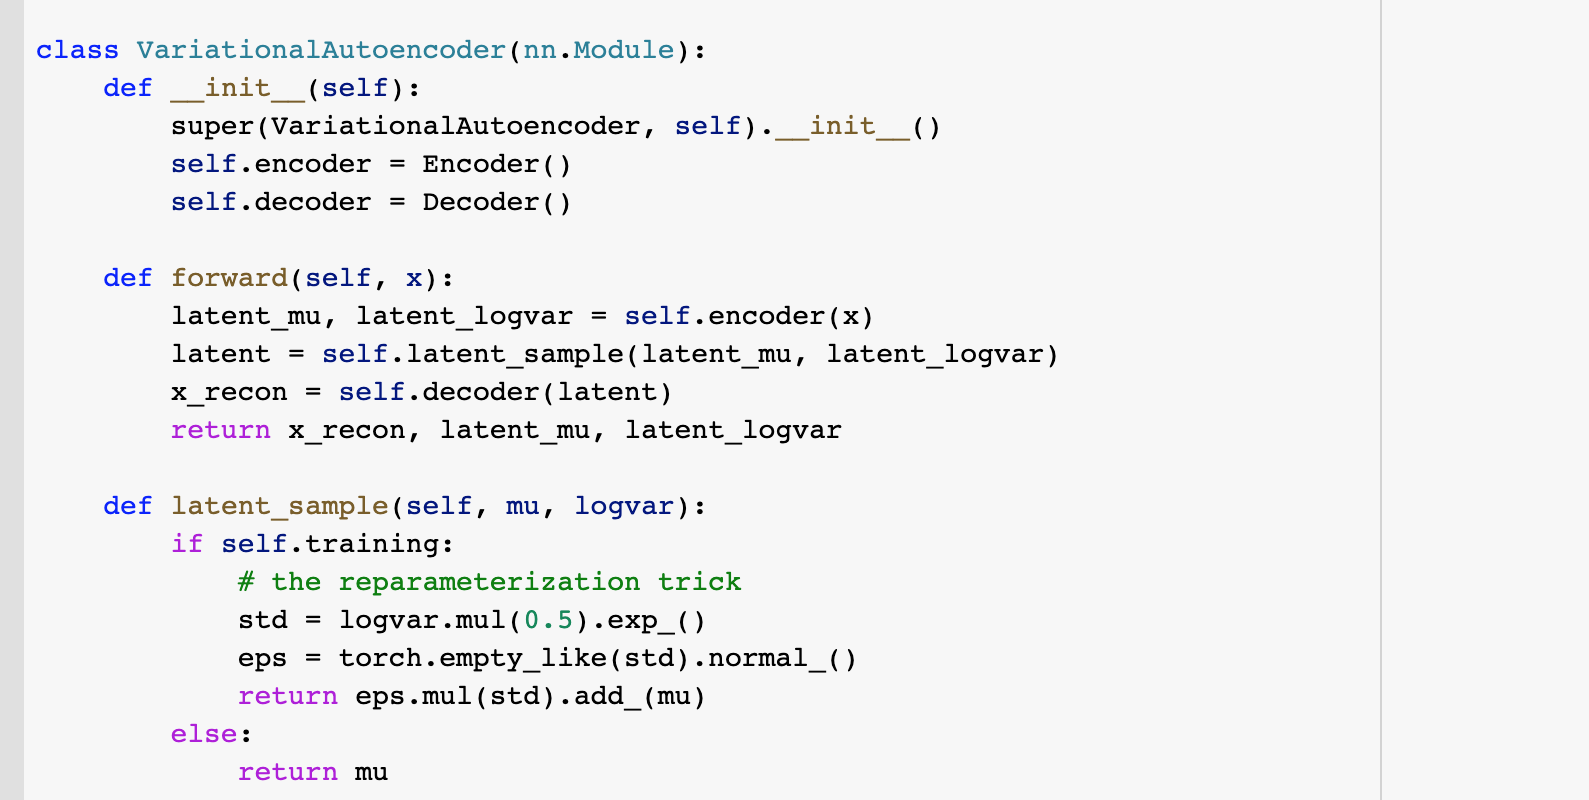
\includegraphics[width=15cm, height=8cm]{vae.png}\\\\The loss function of the variational autoencoder is the negative log-likelihood with a regularizer. The loss function l$_i$ for datapoint x$_i$ is :\\\\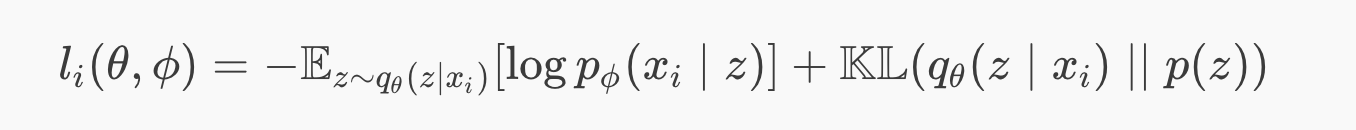
\includegraphics[width=13cm, height=1cm]{loss-function-dia.png}\\The first term is the reconstruction loss, or expected negative log-likelihood of the ith datapoint. The expectation is taken with respect to the encoder’s distribution over the representations. This term encourages the decoder to learn to reconstruct the data.\\The second term is a regularizer . This is the Kullback-Leibler divergence between the encoder’s distribution q$_\theta$(z$\mid$ x) and p(z). This divergence measures how much information is lost  when using q to represent p. It is one measure of how close q is to p.In the variational autoencoder, p is specified as a standard Normal distribution with mean zero and variance one, or p(z) = Normal(0,1)p(z)=Normal(0,1). If the encoder outputs representations z that are different than those from a standard normal distribution, it will receive a penalty in the loss. \\We train the variational autoencoder using gradient descent to optimize the loss with respect to the parameters of the encoder and decoder $\theta$ and $\phi$. For stochastic gradient descent with step size $\rho$, the encoder parameters are updated using $\theta \leftarrow \theta - \rho \frac{\partial l}{\partial \theta}$ and the decoder is updated similarly.\\\\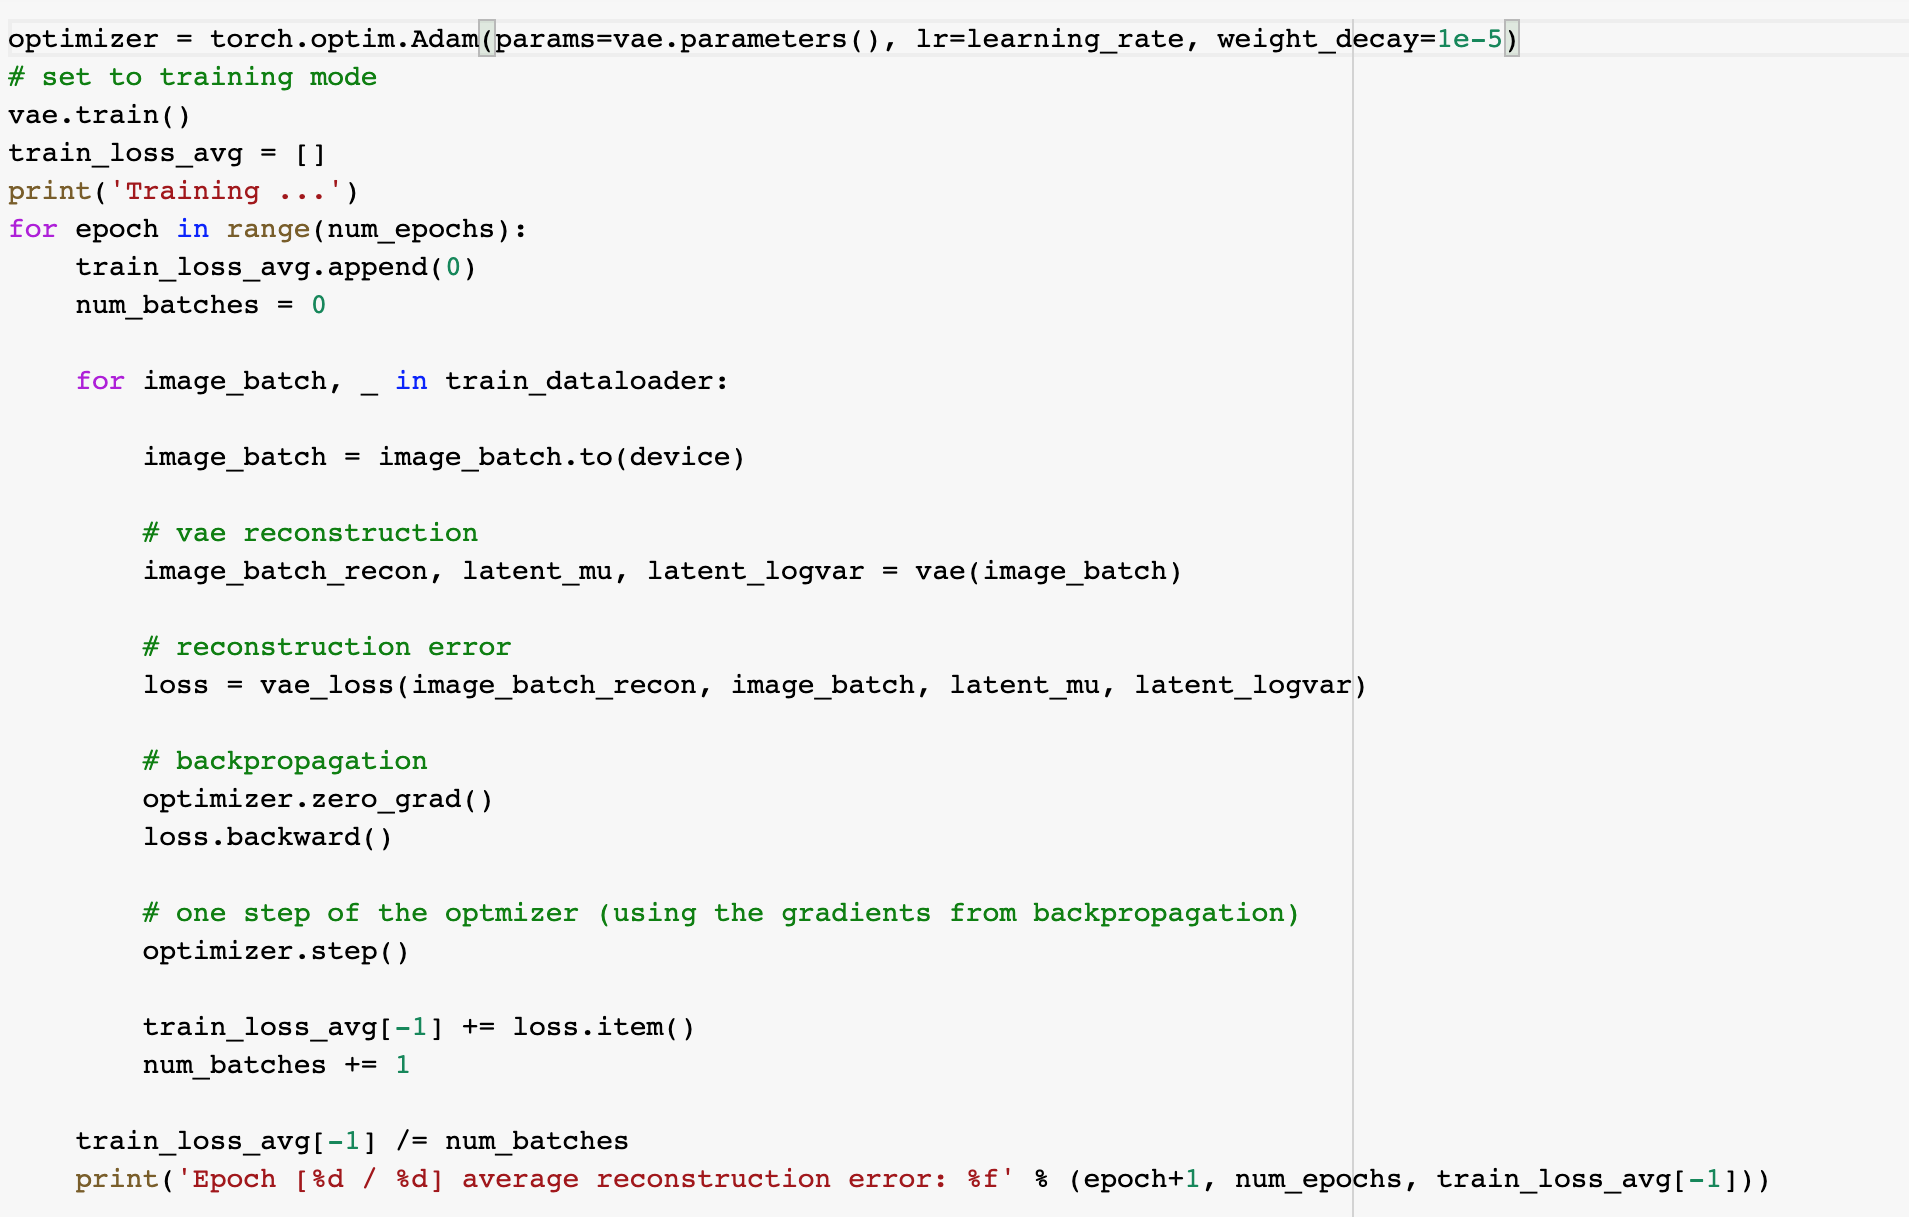
\includegraphics[width=17cm, height=10cm]{train.png}\\\\After training,we observe the reconstruction error decreasing and stabilising as shown:\\\\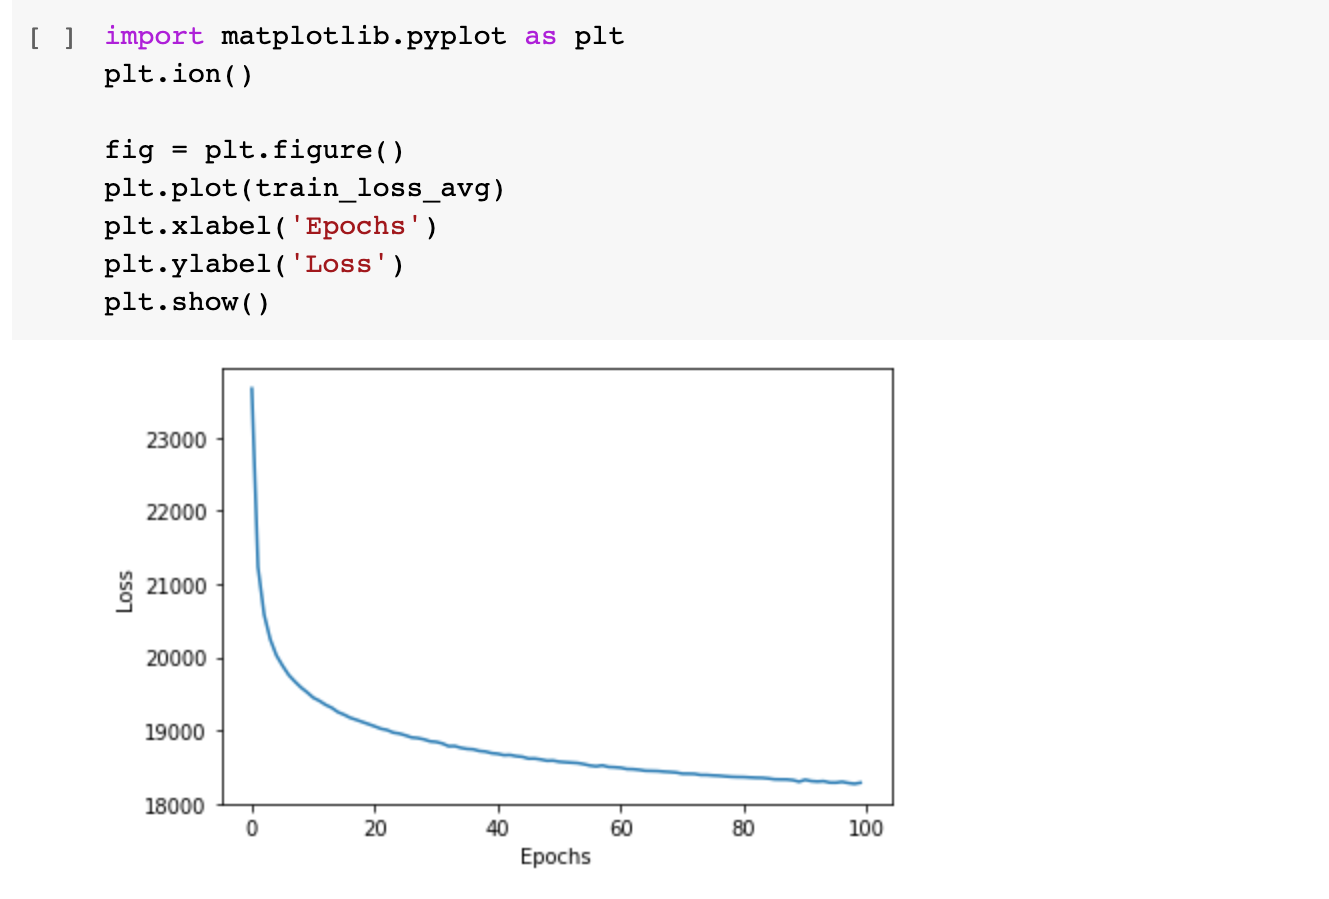
\includegraphics[width=8cm, height=7cm]{plot.png}\\We evaluated on the test set we had initialized earlier and check the reconstruction error : \\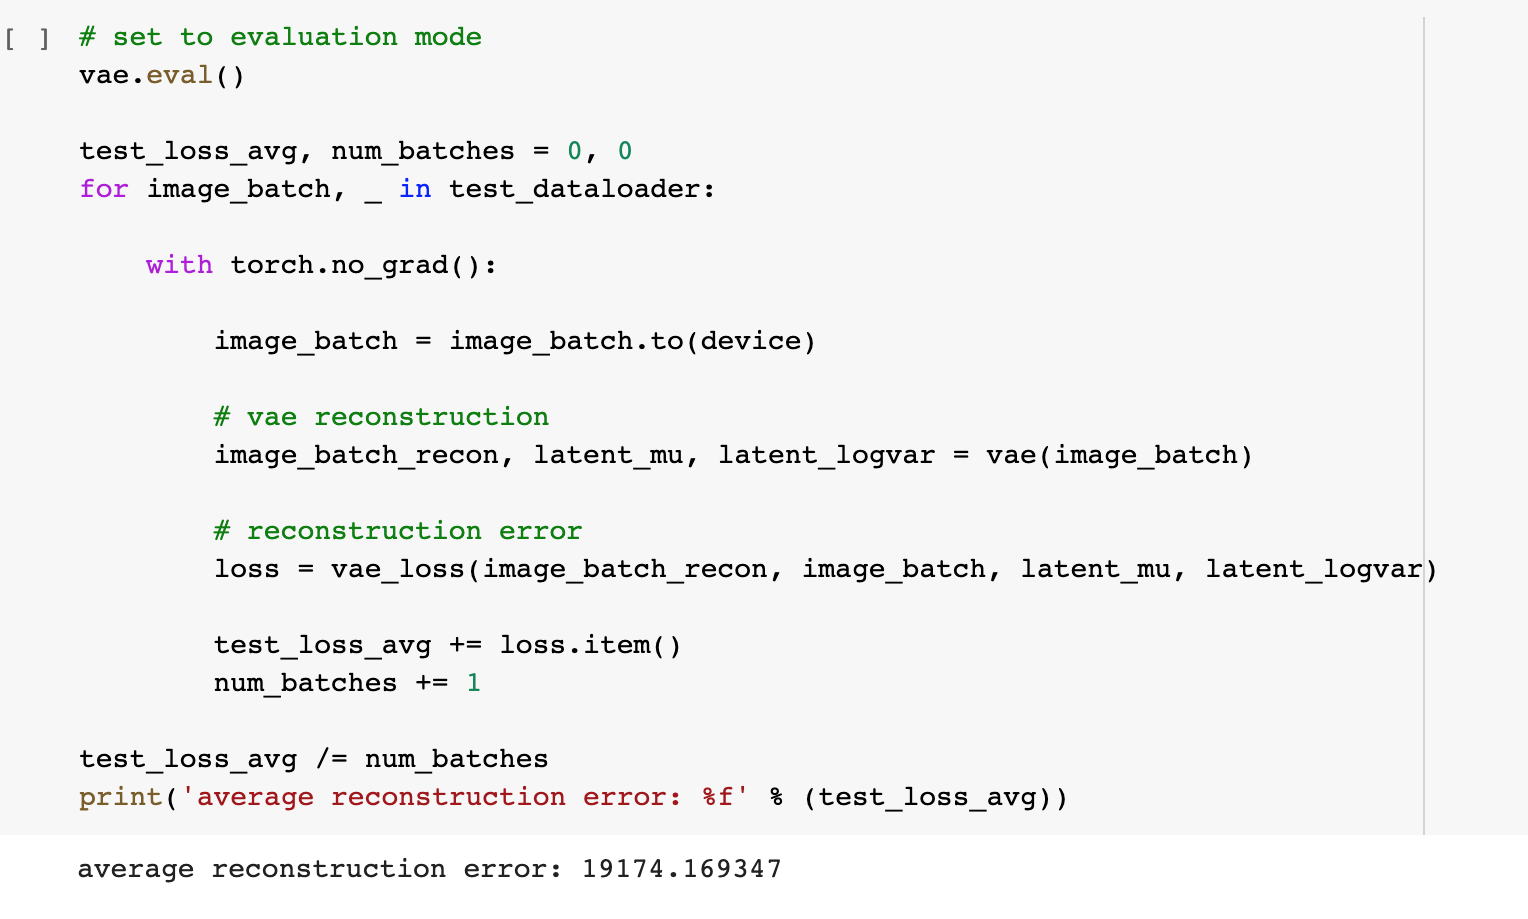
\includegraphics[width=14cm, height=7cm]{eval.png}\\Next, we visualize and compare the reconstruction with our original image. This function takes as an input the images to reconstruct and the name of the model with which the reconstructions are performed. \\\\



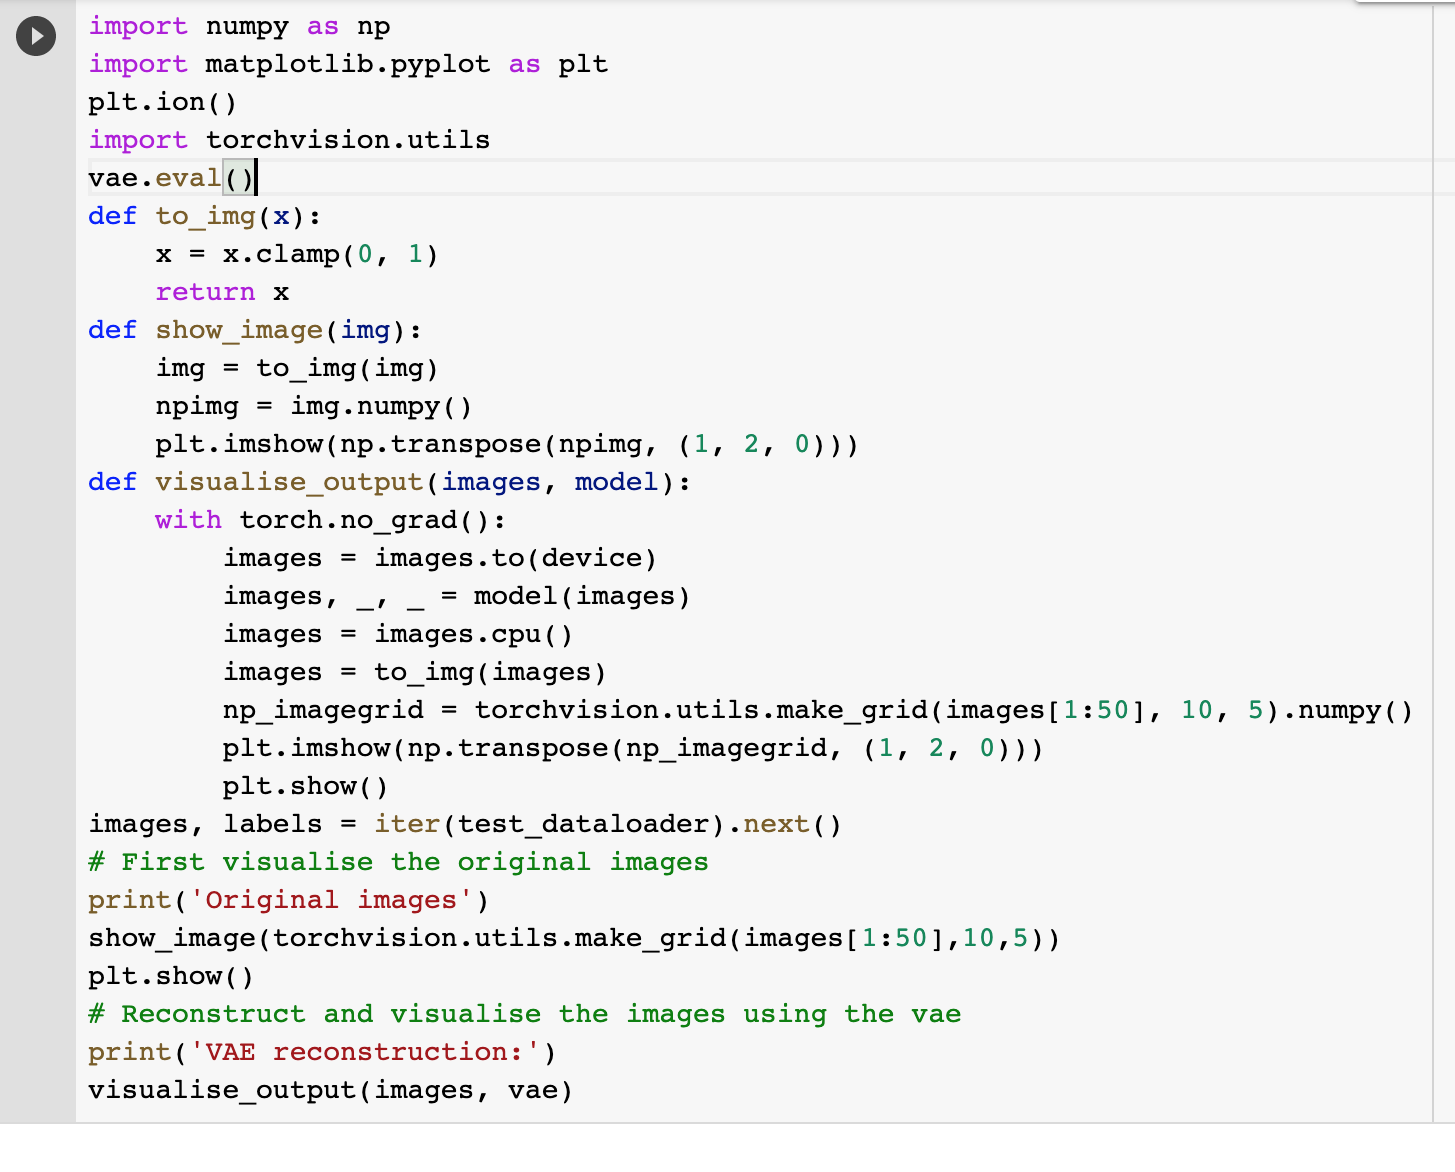
\includegraphics[width=14cm, height=11cm]{recon-code.png}. \\

The results are as follows: \\

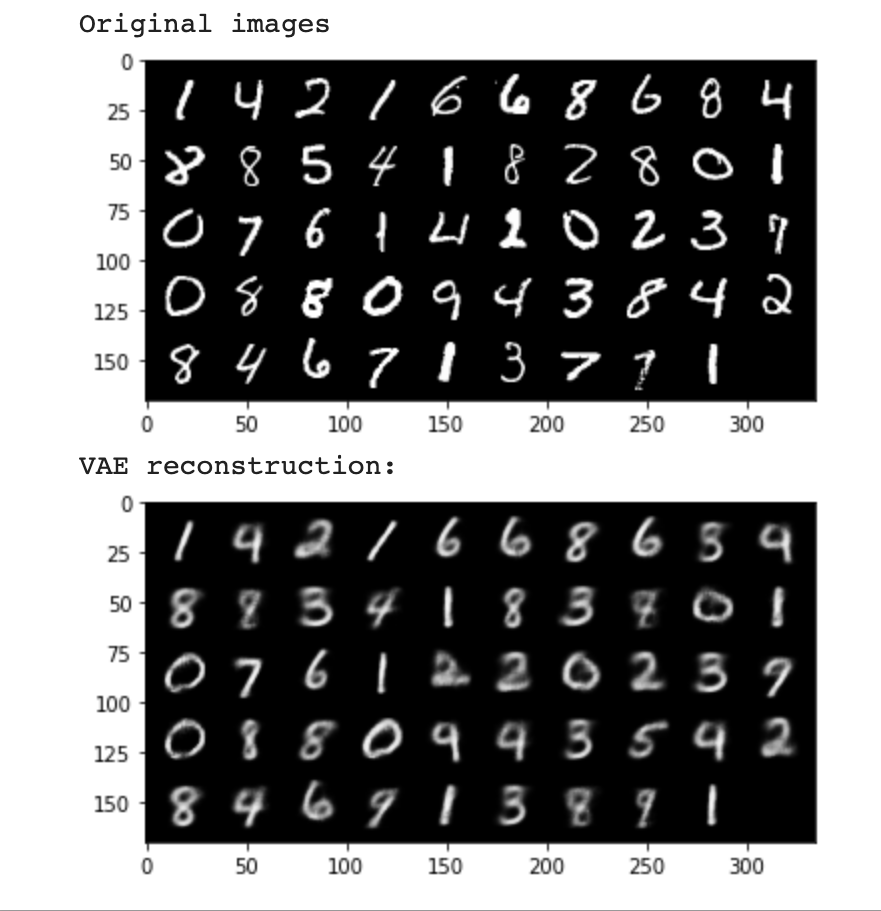
\includegraphics[width=14cm, height=14cm]{recon-result.png}
Link to code : \href{https://colab.research.google.com/drive/1u09z2WUz1U6raMp2rQ5NWROi8bGsD6R_#scrollTo=nzK5YHZJN7gQ}{Colab (Jupyter Notebook)}
\\
\section{Exploratory Data Analysis}
Exploratory Data Analysis on the 20 Newsgroup Dataset can be found here: \href{https://colab.research.google.com/drive/1AJyyKHlCC0zYXFnew3YO8SwZgEECJjvC#scrollTo=pRUpOhY8_wGy}{Colab (Jupyter Notebook)}
\section{Discussion}
Now having an understanding of how variational inference works and implementing a variational autoencoder for MNIST data. We will next recreate the ProdLDA implementation using Pytorch and apply it to 20Newsgroup dataset. 

We will analyse our results and compare them with the paper's implementation, and also make a baseline with LDA. 
\printbibliography
\end{document}
